% --------------------------------------------------------------
% This is all preamble stuff that you don't have to worry about.
% Head down to where it says "Start here"
% --------------------------------------------------------------
 
\documentclass[12pt]{article}
 
\usepackage[margin=1in]{geometry} 
\usepackage{amsmath,amsthm,amssymb}
\usepackage{gensymb}
\usepackage{graphicx}
 
\newcommand{\N}{\mathbb{N}}
\newcommand{\Z}{\mathbb{Z}}
 
\newenvironment{theorem}[2][Theorem]{\begin{trivlist}
\item[\hskip \labelsep {\bfseries #1}\hskip \labelsep {\bfseries #2.}]}{\end{trivlist}}
\newenvironment{lemma}[2][Lemma]{\begin{trivlist}
\item[\hskip \labelsep {\bfseries #1}\hskip \labelsep {\bfseries #2.}]}{\end{trivlist}}
\newenvironment{exercise}[2][Exercise]{\begin{trivlist}
\item[\hskip \labelsep {\bfseries #1}\hskip \labelsep {\bfseries #2.}]}{\end{trivlist}}
\newenvironment{problem}[2][Problem]{\begin{trivlist}
\item[\hskip \labelsep {\bfseries #1}\hskip \labelsep {\bfseries #2.}]}{\end{trivlist}}
\newenvironment{question}[2][Question]{\begin{trivlist}
\item[\hskip \labelsep {\bfseries #1}\hskip \labelsep {\bfseries #2.}]}{\end{trivlist}}
\newenvironment{corollary}[2][Corollary]{\begin{trivlist}
\item[\hskip \labelsep {\bfseries #1}\hskip \labelsep {\bfseries #2.}]}{\end{trivlist}}
 
\begin{document}
\providecommand{\e}[1]{\ensuremath{\times 10^{#1}}}
% --------------------------------------------------------------
%                         Start here
% --------------------------------------------------------------
 
\title{HW 1}%replace X with the appropriate number
\author{Levon Dovlatyan, SI: 24451582\\ %replace with your name
E45} %if necessary, replace with your course title
 
\maketitle
 
\begin{problem}{6.1} %You can use theorem, exercise, problem, or question here.  Modify x.yz to be whatever number you are proving
The following three $\sigma - \epsilon$ data points are provided for a titanium alloy for aerospace. Calculate E for this alloy.
\end{problem}
 
The following three $\sigma - \epsilon$ data points are provided for a titanium alloy for aerospace. Calculate E for this alloy.
%Note 1: The * tells LaTeX not to number the lines.  If you remove the *, be sure to remove it below, too.
%Note 2: Inside the align environment, you do not want to use $-signs.  The reason for this is that this is already a math environment. This is why we have to include \text{} around any text inside the align environment.
\begin{align*}
\epsilon & = 0.002778 \, (\sigma = 300 MPa)\\ 
\epsilon & = 0.005556 \, (\sigma = 600 MPa)\\
\epsilon & = 0.009897 \, (\sigma = 900 MPa)\\
\end{align*}
Plotting the data points given in a strain vs stress plot, we see where the slope changes, and where the actual modulus of elasticity is.
\begin{center}
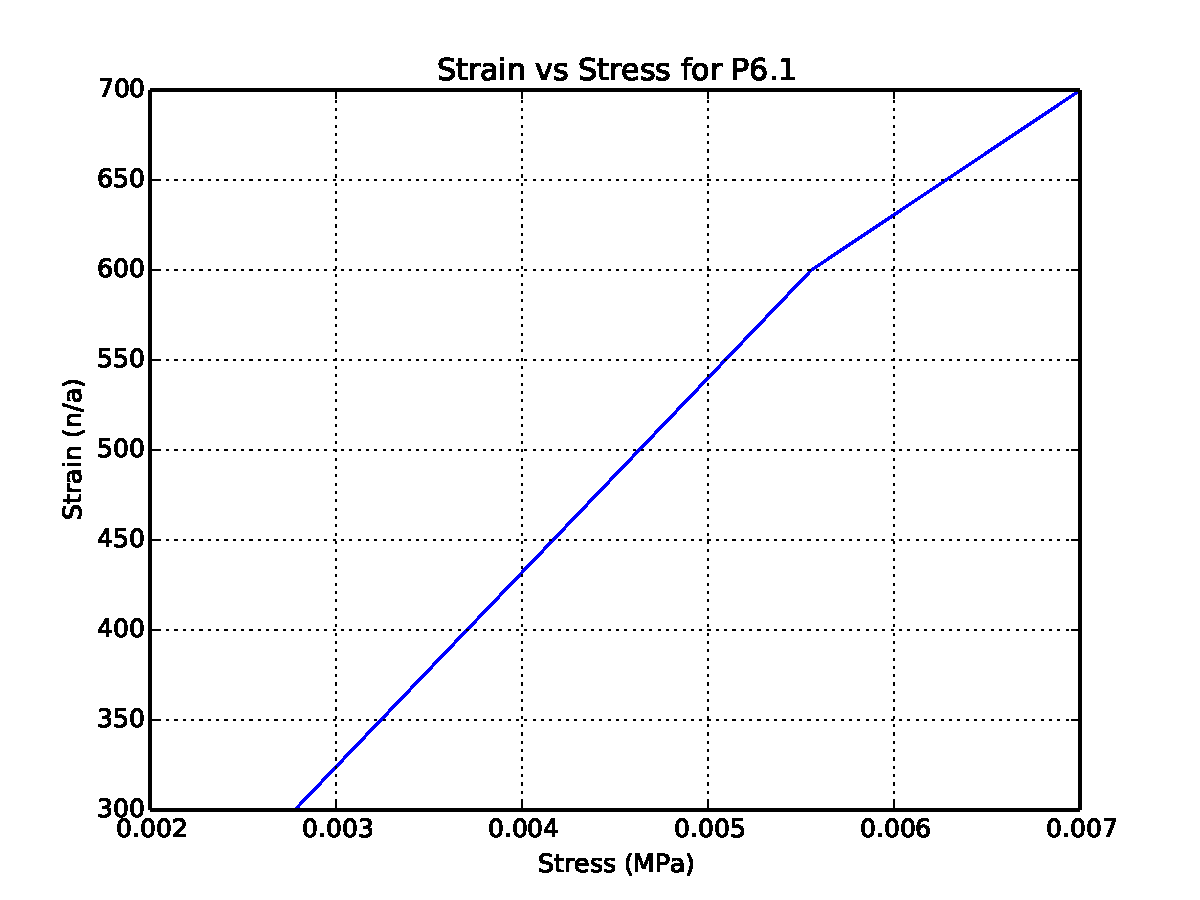
\includegraphics[height=150pt]{graph_p6_1.pdf}
\end{center}
Using the graphical version of Hooke's law, $\sigma = E\epsilon$, we can solve for the modulus E.
\begin{align*}
E = \frac{\sigma}{\epsilon} = \frac{600 \e{6} Pa}{0.005556} = 1.0799 \e{11} \, Pa = 108 \, GPa\\
\end{align*}

\begin{problem}{6.2}
If the Poisson's ration for the alloy in P6.1 is 0.35, calculate \textbf{(a)} the shear modulus G, and \textbf{(b)} the shear stress $\tau$ necessary to produce an angular displacement $\alpha$ of $ 0.2865\degree$.
\end{problem}

\textbf{(a)} Use the following equation for small strains:
\begin{align*}
E & = 2G(1 + \upsilon)\\
G & = \frac{E}{2(1 + \upsilon)} = \frac{1.0799 \e{11} Pa}{2(1 + 0.35)} = 4.00 \e{10} Pa = 40 \, GPa
\end{align*}

\textbf{(b)} Use the following equations for the shear modulus G and the shear strain $\gamma$,
\begin{align*}
\gamma = \tan{\alpha} ,\,\,\, G = \frac{\tau}{\gamma} \\
\tau = G\gamma = G\tan{\alpha} = 4.00 \e{10} Pa * 0.2865\degree * \frac{\pi}{180} = 2.0 \e{8} = 0.2 \, GPa
\end{align*}

\begin{problem}{6.4}
Consider the 1040 carbon steel listed in Table 6.1. \textbf{(a)} A 20-mm-diameter bar of this alloy is used as a structural member in an engineering design. The unstressed length of the bar is precisely 1m. The structural load on the bar is $9 \e{4} N$ in tension. What will be the length of the bar under this structural load? \textbf{(b)} A design engineer is considering a structural change that will increase the tensile load on this member. What is the maximum tensile load that can be permitted without producing extensive plastic deformation of the bar? Give your answer in both newtons (N) and pounds force ($lb_f$).
\end{problem}

\textbf{(a)} To solve for the length of the bar under the structural load, $l$, we can use the equation $\epsilon = \frac{l-l_0}{l_0}$ where $\epsilon$ is the engineering strain and $l_0$ is the length of the unstretched bar. To solve for $\epsilon$ we can use Hook' law, $\sigma = E\epsilon$, and the relationship $\sigma = \frac{P}{A_0}$ where $\sigma$ is the engineering stress, $P$ is the load on the sample, and $A_0$ is the cross sectional area of the 1040 carbon steel.

\begin{align*}
\frac{l-l_0}{l_0} = \epsilon = \frac{\sigma}{E} = \frac{P}{A_0 E} = \frac{4P}{\pi d^2 E} \\
\end{align*}
Rewriting and solving for $l$ where $P = 9 \e{4} N, l_0 = 1m, d = 20 \e{-3}m,$ and $E = 200 \e{9} Pa$
\begin{align*}
l = \frac{4 P l_0}{\pi d^2 E} + l_0 = \frac{4*9 \e{4} N*1m}{\pi * 400 \e{-6}m^2 * 200 \e{9} Pa} + 1m = 1.00143 m 
\end{align*}

\textbf{(b)} Anything above the yield strength starts to deform the bar. Using the equation $\sigma = \frac{P}{A_0}$ and the value of the yield strength for carbon 1040, we can solve for the maximum load.
\begin{align*}
P = \sigma A_0 = 600 \e{6} Pa * \pi 100 \e{-6} m^2 = 1.88 \e{5} N
\end{align*}
Using the conversion of $1 lb_f = 4.448 N$, we see that $P = 1.88 \e{5} N * \frac{0.2248 \, lb_f}{N} = 4.24 \e{4}\, lb_f$.

\begin{problem}{6.16}
A single crystal $Al_2O_3$ rod (precisely 6mm diameter x 50 mm long) is used to apply loads to small samples in a high-precision dilatometer (a length-measuring device). Calculate the resultign rod dimension if the crystal is subjected to a 25-kN axial compression load.
\end{problem}

To solve for $l_x$ using the engineering strain equation, $l_x = l_0\,(1 + \epsilon)$. Also since this is axial compression, the force P must be negative.
\begin{align*}
l_x & = l_0 (1 + \epsilon) = l_0 (1 + \frac{\sigma}{E}) = l_0 (1 + \frac{-P}{A_0 E}) = l_0 (1 + \frac{-P}{\pi r^2 E}) \\ 
& = 50 \e{-3}m (1 + \frac{-25 \e{3} N}{\pi * 9 \e{-6}m^2 * 380 \e{9} Pa}) \\
& = 49.88 \, mm
\end{align*}
To solve for the diameter expansion, $l_y$ we use the Poisson's ratio to solve for $\epsilon_y$
\begin{align*}
l_y = l_0 (1 + \epsilon_y) = l_0 (1 - \epsilon_x \upsilon)
\end{align*}
Note that $\upsilon = 0.26$ and that $\epsilon_x = \frac{-P}{\pi r^2 E} = -2.33 \e{-3}$ from above.
\begin{align*}
l_y = 6 \e{-3}(1 - (-2.33 \e{-3})0.26) = 6.0036 \, mm
\end{align*}

\begin{problem}{6.45}
You are asked to measure nondestructively the yield strength and tensile strength of an annealed 65-45-12 cast iron structural member. Fortunately, a small hardness indentation in this structural design will not impair its future usefulness, which is a working definition of nodestructive. A 10-mm-diameter tungsten carbide sphere creates a 4.26-mm-diameter impression under a 3,000-kg load. What are the yield and tensile strengths?
\end{problem}

Use the sphere hardness equation in table 6.9, where P = 3000kg, D = 10 mm, d = 4.26 mm
\begin{align*}
BHN & = \frac{2P}{\pi D(D - \sqrt{D^2 - d^2})} = \frac{2(3000kg)}{\pi 10mm(10mm - \sqrt{10^2mm - 4.26^2mm})} \\
& \approx 200
\end{align*}
Using the graph in figure 6.29b, a BHN of 200 produces a yield strength of about 400 and a tensile strenth of about 550.
% --------------------------------------------------------------
%     You don't have to mess with anything below this line.
% --------------------------------------------------------------
 
\end{document}
